\newthought{\textbf{Adinda Awaliah - 2020903430004 - TRKJ 3B}}

\newday{\textbf{15 september 2022}}
\begin{enumerate}
\item Kendala dan Solusi
% jelaskan kendala dan penyebab yang dialami saat mengikuti praktikum serta solusi atau langkah-langkah yang telah dilakukan
\newline praktikum instalasi apache hadoop tidak ada kendala.

\item Kesimpulan
% berikan kesimpulan dari praktikum yang telah dikerjkan
\newline berhasil melakukan instalasi.

\begin{figure}
\setlength{\belowcaptionskip}{-10pt}
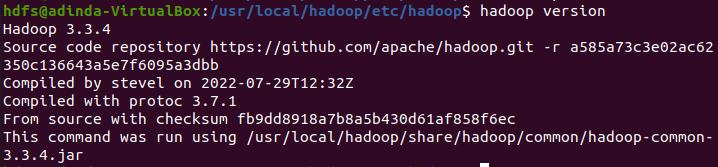
\includegraphics[width=\textwidth]{AdindaAwaliah/hasil instalasi apache hadoop}
\caption{Versi Java yang Terinstall}
\label{gam:hasil instalasi apache hadoop}
\end{figure}

\end{enumerate}

\newday{\textbf{1 desember 2022}}
\begin{enumerate}
\item Kendala dan Solusi
% jelaskan kendala dan penyebab yang dialami saat mengikuti praktikum serta solusi atau langkah-langkah yang telah dilakukan

\item Kesimpulan
% berikan kesimpulan dari praktikum yang telah dikerjkan

\end{enumerate}

\newday{\textbf{02 desember 2022}}
\begin{enumerate}
\item Kendala dan Solusi
% jelaskan kendala dan penyebab yang dialami saat mengikuti praktikum serta solusi atau langkah-langkah yang telah dilakukan

\item Kesimpulan
% berikan kesimpulan dari praktikum yang telah dikerjkan

\end{enumerate}

\newday{\textbf{08 desember 2022}}
\begin{enumerate}
\item Kendala dan Solusi
% jelaskan kendala dan penyebab yang dialami saat mengikuti praktikum serta solusi atau langkah-langkah yang telah dilakukan

\item Kesimpulan
% berikan kesimpulan dari praktikum yang telah dikerjkan

\end{enumerate}

\newday{\textbf{09 desember 2022}}
\begin{enumerate}
\item Kendala dan Solusi
% jelaskan kendala dan penyebab yang dialami saat mengikuti praktikum serta solusi atau langkah-langkah yang telah dilakukan

\item Kesimpulan
% berikan kesimpulan dari praktikum yang telah dikerjkan

\end{enumerate}

\newday{\textbf{15 desember 2022}}
\begin{enumerate}
\item Kendala dan Solusi
% jelaskan kendala dan penyebab yang dialami saat mengikuti praktikum serta solusi atau langkah-langkah yang telah dilakukan

\item Kesimpulan
% berikan kesimpulan dari praktikum yang telah dikerjkan

\end{enumerate}

\newday{\textbf{16 desember 2022}}
\begin{enumerate}
\item Kendala dan Solusi
% jelaskan kendala dan penyebab yang dialami saat mengikuti praktikum serta solusi atau langkah-langkah yang telah dilakukan

\item Kesimpulan
% berikan kesimpulan dari praktikum yang telah dikerjkan

\end{enumerate}

